\chapter{Terrain Classification for AMOS II} \label{chapter:05:terrain_classification}
Classification, one of the most widely used areas of machine learning, has a broad array of applications (see \cref{chapter:01:introduction}). To fit a classifier to a problem, one needs to define a problem data structure. Data consists of samples and discrete targets, often called classes. The samples are sooner or later converted into so called feature vectors of a specified length. The lenght of feature vectors usually determines an input of chosen classifier and number of classes sets an output.

Out of a wide range of classification methods, a feedforward neural network approach (see \cref{chapter:04:neural_net_implementation}) is chosen. The classification problem is connected to AMOS II, an open-source multi sensori-motor robotic platform. The task is to classify various terrain types, while the only input comes from proprioceptive sensors. The overall process is based on simulation data.

\section{Overall process summary}
The very first step is to make the AMOS II simulation run (\cref{ssec:lpzrobots_sim}). Then a simple tripod gait controller is implemented. To generate various terrain types, the number of variable terrain quailities and their ranges are determined (\cref{ssec:terrain_qualities}). Based on these qualities (parameters), a number of virtual terrains is defined (\cref{ssec:terrain_parameters}) and an optimality of these parameters is briefly analysed (\cref{ssec:terrains_analysis}).

Next, AMOS II (its simulation alternative) is forced to walk on every defined terrain type for a sufficiently long period of time and data from all proprioceptive sensors is saved. This data is then verified and failing experiments are removed. The data acquisition step is parameterized by a standard deviation of additive (Guassian) terrain noise and is run for several values.

Having a clean simulation data from all sensors, a feature vector structure is determined. Then a Gaussian signal noise is added. Finally, a dataset is created by splitting all the data into training, validation and testing sets. It is indicated on \cref{img:terrain_classification_process}, that several datesets and several classifiers are generated during the process. These packages may differ in following parameters.

\textit{Dataset parameters:}
\begin{itemize}
\item terrain types included
\item sensors on input
\item samples length (number of simulation timesteps)
\item terrain noise
\item signal noise
\item number of samples
\end{itemize}

\textit{Trained net parameters:}
\begin{itemize}
\item neural network structure
\item accuracy on training/validation/testing sets 
\end{itemize}

An optimal neural network classifier is found. The optimal network is then pruned by the algorithm developed in section X. Classification performance of developed tools are compared to a \textit{Scikit-learn} network classification library sknn [].

\begin{figure}[H]
  \centering
  \includegraphics[width=1.0\textwidth]{terrain_classification_process}
  \caption{Terrain classification process - overall diagram.}
  \label{img:terrain_classification_process}
\end{figure}

\section{Experimental Environment Specification}
target machine description

3-5 pages

\subsection{Hexapod Robot AMOS II}

\begin{figure}[H]
  \centering
  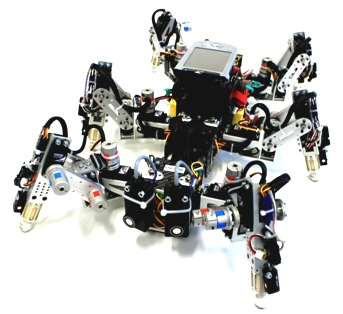
\includegraphics[width=343px]{amosii}
  \caption{AMOS II.}
  \label{img:amosii}
\end{figure}

\subsection{LPZ Robots Simulation} \label{ssec:lpzrobots_sim}
It is a part of a simulation software called \textit{LpzRobots} provided by the University of Leipzig \citep{misc:lpzrobots} under GPL license.

\section{Virtual Terrain types}
Since the verification is based on the simulation only, the goal is to design an authentical virtual environment. For this purpose various terrain types need to be virtually imitated.

Luckily, the \textbf{LpzRobots} AMOS II simulator supports some terrain settings. In the main simulation file (\textit{main.cpp} - see \ref{app:code_documentation}), a \textit{'rough terrain'} substance is being initialized and passed through a handle to a \textit{TerrainGround} constructor.

\begin{lstlisting}[language=C++, caption={Setting a terrain ground in main.cpp}, label=code:terrain_ground]
Substance roughterrainSubstance(terrain_roughness, terrain_slip,
                       terrain_hardness, terrain_elasticity);
oodeHandle.substance = roughterrainSubstance;
TerrainGround* terrainground = new TerrainGround(oodeHandle, 
                       osgHandle.changeColor(terrain_color),
                       "rough1.ppm", "", 20, 25, terrain_height);
\end{lstlisting}

As \cref{code:terrain_ground} shows, the terrain substance is defined by four parameters: \textbf{roughness}, \textbf{slipperiness}, \textbf{hardness} and \textbf{elasticity}.

Besides the substance handle, the \textit{TerrainGround} constructor takes six more arguments.

\begin{description}
\item[terrain\_color] : simulation ground color
\item["rough1.ppm"] : an image in the .ppm format, a lowest common denominator color image file format \citep{misc:ppm}, a bitmap height file
\item[""] : texture image (not used)
\item[20] : walking area x-size 
\item[25] : walking area y-size
\item[terrain\_height] : maximum terrain height
\end{description}

\subsection*{Terrain qualities} \label{ssec:terrain_qualities}
Out of the listed ground parameters, some of them are picked up and being called \textit{terrain qualities}, as they define a specific terrain type.

It has been decided not to change the \textit{.ppm} image for various terrains and so \textit{rough1.ppm} is fixed. Also the walking area is set to (big enough) final size of \textit{20x25}. The color is variable, however, besides the simulation graphics it does not have any effect on results. 

Therefore, a virtual terrain type is defined by five qualitites. Each of them is a float number from an empirically stated range \footnote{The upper range limits have been set up based on significant changes in robot behaviour for various parameter values.}. (\cref{tab:terrain_qualities}).

\begin{table}[H]
\centering
\caption{Terrain qualities and their ranges}
\label{tab:terrain_qualities}
\begin{tabular}{lccll}
             & min value & max value \\
roughness    & 0.0       & 10.0      \\
slipperiness & 0.0       & 100.0     \\
hardness     & 0.0       & 100.0     \\
elasticity   & 0.0       & 2.0       \\
height       & 0.0       & 0.1 
\end{tabular}
\end{table}

\subsection*{Terrains parameters determination} \label{ssec:terrain_parameters}
To determine a terrain type, one has to come up with the five parameters from \cref{tab:terrain_qualities}.

First, number of identifiable virtual terrain types needs to be determined. For purposes of this thesis, it has been decided to create \textbf{14 terrain types}. Their parameters (showed in \cref{tab:terrains_parameters}) have been set up intuitively, based on the AMOS II simulated behaviour. With respect to the qualities ranges from \cref{tab:terrain_qualities}, the values have been normed to (0, 1).

\begin{table}[H]
\centering
\caption{Virtual terrain types parameters.}
\label{tab:terrains_parameters}
\begin{tabular}{|l|l|c|c|c|c|c|}
\hline
\textit{\#}                                       & \textit{terrain title} & \multicolumn{1}{l|}{\textit{roughness}} & \multicolumn{1}{l|}{\textit{slipperiness}} & \multicolumn{1}{l|}{\textit{hardness}} & \multicolumn{1}{l|}{\textit{elasticity}} & \multicolumn{1}{l|}{\textit{height}} \\ \hline
\cellcolor[HTML]{876496}1                         & \textbf{carpet}        & 0.3                                     & 0.0                                        & 0.4                                    & 0.15                                     & 0.2                                  \\ \hline
\cellcolor[HTML]{9C9FA6}2                         & \textbf{concrete}      & 1.0                                     & 0.0                                        & 1.0                                    & 0.0                                      & 0.0                                  \\ \hline
\cellcolor[HTML]{DCE696}3                         & \textbf{foam}          & 0.5                                     & 0.0                                        & 0.0                                    & 1.0                                      & 0.7                                  \\ \hline
\cellcolor[HTML]{239614}4                         & \textbf{grass}         & 0.5                                     & 0.0                                        & 0.3                                    & 0.3                                      & 0.5                                  \\ \hline
\cellcolor[HTML]{737F9C}5                         & \textbf{gravel}        & 0.7                                     & 0.001                                      & 1.0                                    & 0.0                                      & 0.3                                  \\ \hline
\cellcolor[HTML]{D7E3FF}6                         & \textbf{ice}           & 0.0                                     & 1.0                                        & 1.0                                    & 0.0                                      & 0.0                                  \\ \hline
\cellcolor[HTML]{646464}7                         & \textbf{mud}           & 0.05                                    & 0.05                                       & 0.005                                  & 0.25                                     & 0.2                                  \\ \hline
\cellcolor[HTML]{96FABE}8                         & \textbf{plastic}       & 0.1                                     & 0.02                                       & 0.6                                    & 0.5                                      & 0.0                                  \\ \hline
\cellcolor[HTML]{6E5A3C}9                         & \textbf{rock}          & 1.0                                     & 0.0                                        & 1.0                                    & 0.0                                      & 1.0                                  \\ \hline
\cellcolor[HTML]{000000}{\color[HTML]{FFFFFF} 10} & \textbf{rubber}        & 0.8                                     & 0.0                                        & 0.8                                    & 1.0                                      & 0.0                                  \\ \hline
\cellcolor[HTML]{F2EE7C}11                        & \textbf{sand}          & 0.1                                     & 0.001                                      & 0.3                                    & 0.0                                      & 0.2                                  \\ \hline
\cellcolor[HTML]{FDB0FB}12                        & \textbf{snow}          & 0.0                                     & 0.8                                        & 0.2                                    & 0.0                                      & 0.2                                  \\ \hline
\cellcolor[HTML]{324B32}13                        & \textbf{swamp}         & 0.0                                     & 0.05                                       & 0.0                                    & 0.0                                      & 1.0                                  \\ \hline
\cellcolor[HTML]{5A4100}14                        & \textbf{wood}          & 0.6                                     & 0.0                                        & 0.8                                    & 0.1                                      & 0.2                                  \\ \hline
\end{tabular}
\end{table}

Colors linked to the terrains in \cref{tab:terrains_parameters} are used in the simulation as well as in the figures in Results section.

\subsection*{Analysis of chosen parameters} \label{ssec:terrains_analysis}
In general, proper data preparation is an important part of classification tasks, hence a brief analysis is presented.

The goal is to imitate real terrains authentically as possible and at the same time to generate such terrains, that are clearly distinguishable from each other. The more two terrains differ the better classification results are expected.

Having five terrain qualities calls for a 5-D space, which is difficult to illustrate or even imagine. Therefore, formula \ref{eq:similarity_factor} is used to compute a similarity factor of two terrain types (the five qualities are listed in \cref{tab:terrain_qualities} and \cref{tab:terrains_parameters}).


\begin{equation} 
\label{eq:similarity_factor}
  SF_{t_1, t_2} = \displaystyle\sum_{i=1}^{5} \abs{quality(i, t_1) - quality(i, t_2)}
\end{equation} 

Naturally, equation \ref{eq:similarity_factor} ends up with $ SF_{similar} = 0.0 $ for two terrains with exactly same parameters and $ SF_{different} = 5.0 $ for two terrains differing most possibly.

The following figure (\ref{fig:terrains_parameters}) shows the variability (similarity factors) of generated terrains.

\begin{figure}[H]
  \centering
  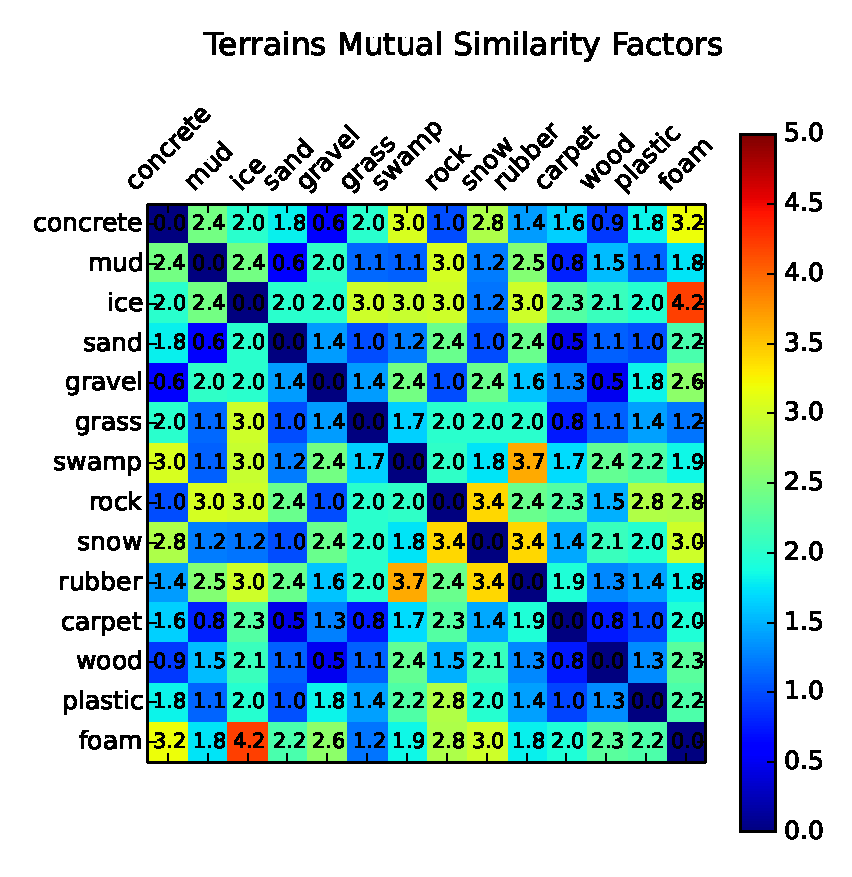
\includegraphics[width=1.0\textwidth]{terrains_variability.eps}
  \caption{Variability of generated terrain types.}
  \label{fig:terrains_parameters}
\end{figure}


\section{Net Input Fixation}
Determination of sensors to be used and its transformation into a feature vector

2-3 pages

\section{Data Acquisition}
Description of how the data has been acquired from the simulation and saved as .txt, adding terrain noise

2 pages
\subsection{Terrain Noise}

\section{Data Processing}
Cleaning the data (deleting incomplete ones), adding signal noise, transformation into datasets, splitting into training-validation-testing sets

2-3 pages
\subsection{Signal Noise}

\section{Training and Classification}

Neural net training with several parameters and comparison with training with scikit-neuralnetwork library

2-3 pages

\subsection{Scikit-neuralnetwork library}
brief description of the library and its usage 1/2 pages

1 page